\documentclass[12pt]{article}
\usepackage{graphicx}
\usepackage[dutch]{babel}
\usepackage{amsmath,amsthm,amssymb}
\usepackage{array}
\usepackage[table,xcdraw]{xcolor}
\usepackage{float}
\usepackage[normalem]{ulem}
\usepackage{tcolorbox}
\usepackage{xcolor}
\usepackage[margin=1in]{geometry}
\usepackage{tikz}
\DeclareMathOperator{\R}{\mathbb{R}}
\DeclareMathOperator{\N}{\mathbb{N}}
\newcommand{\Lim}[1]{\raisebox{0.5ex}{\scalebox{0.8}{$\displaystyle \lim_{#1}\;$}}}

\title{Analyse van de dubbelster BD+39\_4926}
\author{Jul Comhaire (r0980824), Jente Delnoij (r0986085),\\
	Leandro Matthys (r1010158), Mathias Meersschaut (r0998972)}

\begin{document}
	\maketitle
	\tableofcontents
	\pagebreak
	\section{Doelstelling}
	De snelheid en massa van het dubbelstersysteem BD+39\_4926 berekenen door gebruik te maken van observaties van de HERMES spectrograaf.
	\section{Theorie}
	De positie van het massacentrum $x_{MC}$ kan bepaald worden via:
	\begin{equation}
	   	x_{\text{MC}} = \frac{m_1x_1 + m_2x_2}{m_1 + m_2}
	\end{equation}
	Hierin zijn $m_1$ en $m_2$ de massa's van de twee sterren in het dubbelstersysteem en $x_1$ en $x_2$ hun respectievelijke posities.
	\begin{center}
		\begin{minipage}{1\textwidth}
			\begin{figure}[H]
				\centering
				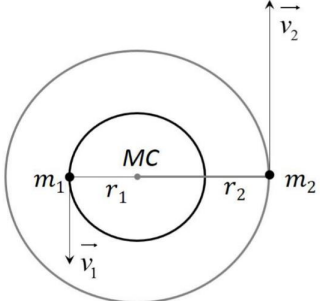
\includegraphics[width=0.3\textwidth]{illustratie_dubbelster.png}
				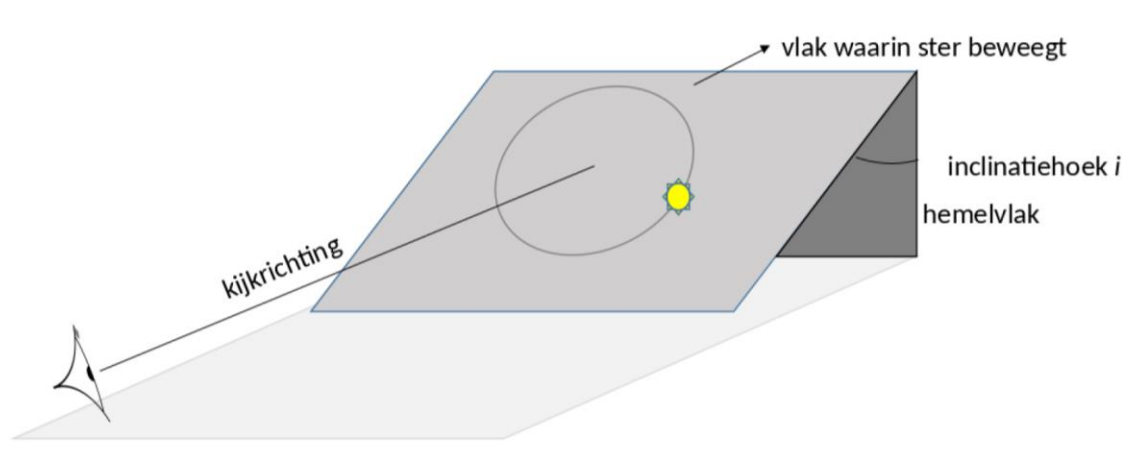
\includegraphics[width=0.6\textwidth]{inclinatiehoek.PNG}
				\caption{Schematische voorstelling van (links) het dubbelstersysteem met $m_1$ en $m_2$ de massa's van de twee sterren en $MC$ het massacentrum, en (rechts) de inclinatiehoek van het vlak waarin het stersysteem beweegt.}
				\label{fig 1:Illustratie_dubbelster}
			\end{figure}
		\end{minipage}
	\end{center}
	Ook zijn volgende formules gebruikt:
	\begin{equation}
	   	|F_{12}| = |F_{21}| = G \cdot \frac{m_1 m_2}{{(r_1 + r_2)}^2} \quad \text{(Gravitatiekracht)}
	\end{equation}
	\\
	\begin{equation}\label{massafunctie}
		 f(M)= \frac{P}{2\pi G}({v_{1r}})^3 = \frac{m_2^3 \sin^3(i)}{(m_1 + m_2)^2} \quad \text{(Massafunctie)}
	\end{equation}
	\\
	\begin{equation}\label{lambda}
		\frac{\lambda - \lambda_0}{\lambda_0} = \frac{v}{c} \quad \text{(Relatieve golflengtefunctie)}
	\end{equation}
	In bovenstaande formules is $P$ de periode van de cirkelbeweging van de geobserveerde ster, $v_{1r}$ de radiale snelheid van deze ster, en $i$ de inclinatie van het hellingsvlak waarin deze sterren bewegen.
	$\lambda_0$ is de uitgezonden golflengte en $\lambda$ is de geobserveerde golflengte.
	\newpage
	\section{Meetopstelling}
Er werd gebruik gemaakt van datasets opgemeten door de HERMES spectrograaf, die gemonteerd staat op de Mercator telescoop op het Canarische eiland La Palma. Deze data bevat de intensiteiten per golflengte op verschillende tijdsstippen. De HERMES spectrograaf heeft 168.000 kanalen over een interval van 390 nm tot 900 nm \label{spectrograaf} \cite{Opgave Sterrenkundeproef}. Hieronder een schematische voorstelling van HERMES.
\begin{figure}[h]
   	\centering
    	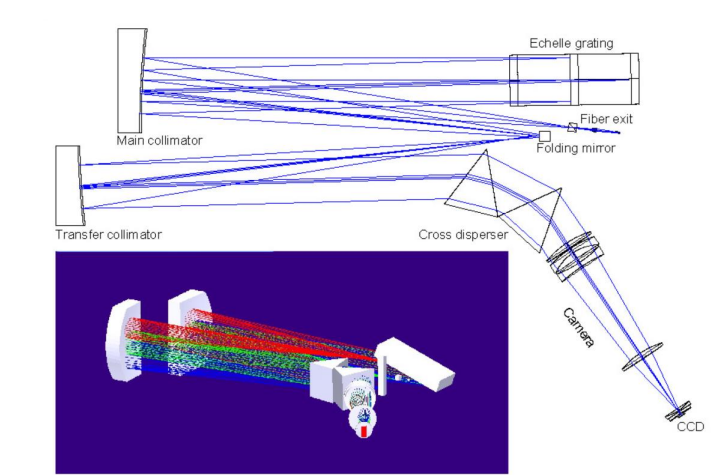
\includegraphics[width=0.6\textwidth]{plagiaat.png}
    	\caption{Optisch ontwerp van de HERMES spectrograaf.}
    	\label{fig 2:HERMES}
\end{figure}

	\section{Meetresultaten}
De volgende figuur toont de intensiteiten per golflengte. Hieruit kan de verschuiving van de absorptielijnen bepaald worden.
\begin{figure}[h]
   	\centering
    	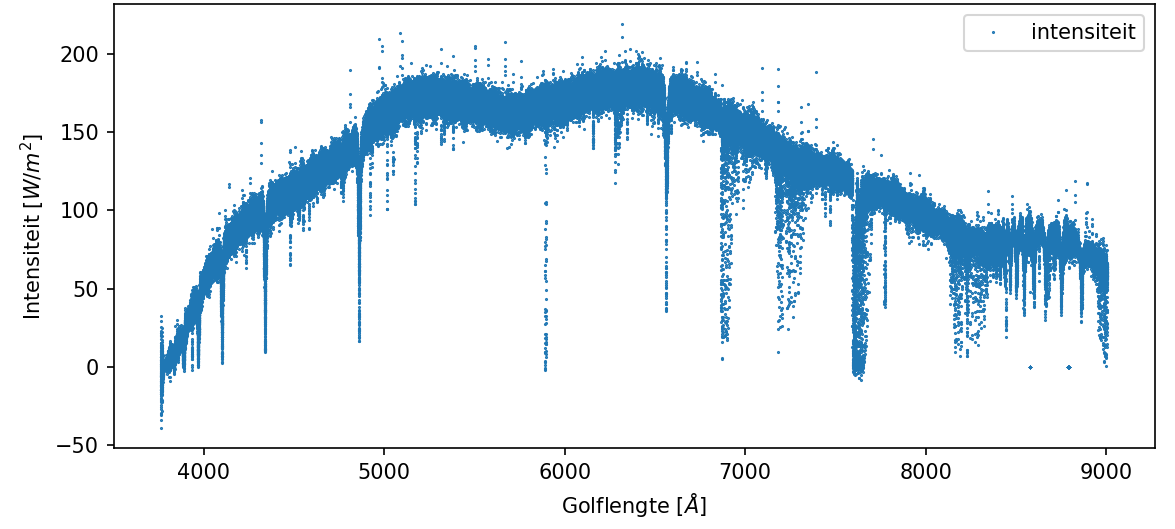
\includegraphics[width=0.8\textwidth]{intensiteit per golflengte.png}
    	\caption{Intensiteit per golflengte.}
    	\label{fig 3:Intensiteit per golflengte.}
\end{figure}


\newpage
	\section{Analyse}
	De radiale snelheid wordt bepaald door de theoretische absorptielijnen te verschuiven volgens de formule van het dopplereffect \eqref{lambda} tot deze samenvallen met de waargenomen absorptielijnen, zichtbaar als lokale minima in het spectrogram. Om de juiste verschuiving te bepalen, wordt de som van de intensiteiten op de verschoven spectraallijnposities geminimaliseerd. Concreet kan dit bekomen worden door een aantal radiale snelheden te overlopen en daarna de som van de intensiteiten van alle verschoven absorptielijnen te minimaliseren. Vervolgens wordt dit resultaat stapsgewijs verfijnd door in te zoomen op een steeds kleiner interval rond het minimum.\\
	Omdat uit deze analyse duidelijk is dat alle spectraallijnen verschoven zijn naar kortere golflengten, gaat het hier om een blauwverschuiving.
	De volgende figuur toont een deel van het spectrum waarop de blauwverschuiving van de absorptielijnen gevisualiseerd wordt.
	\\ 
	\begin{figure}[h]
	   	\centering
	    	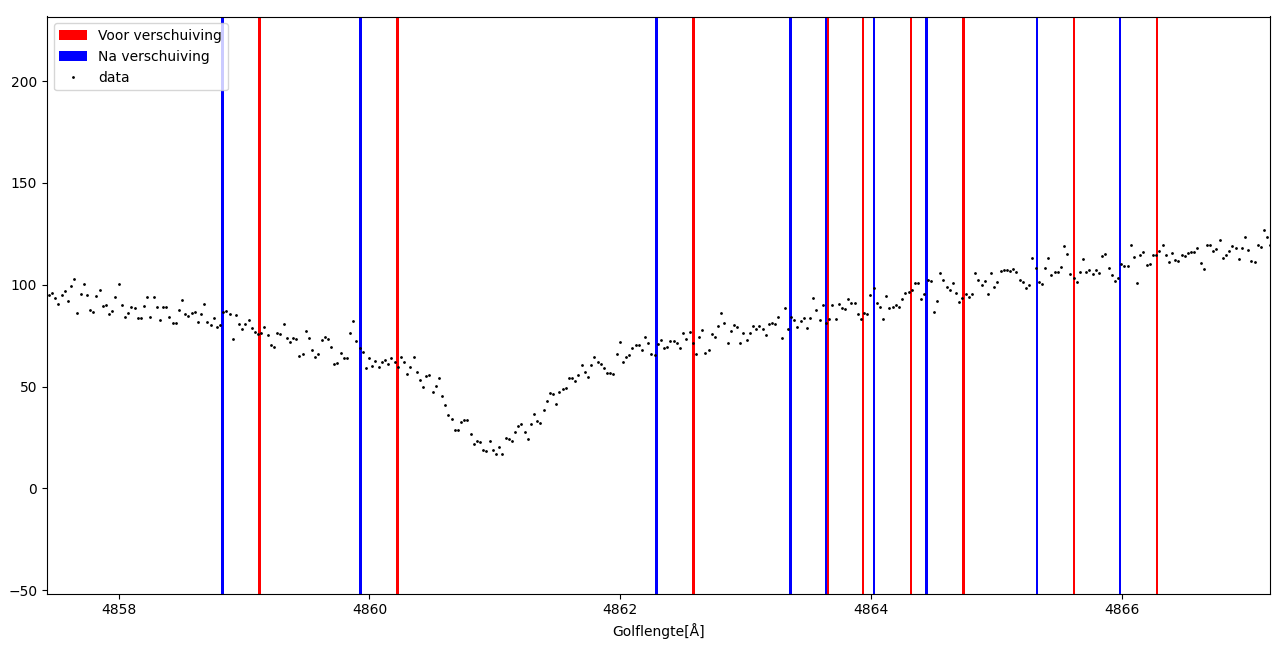
\includegraphics[width=1\textwidth]{shift.png}
	    	\caption{Blauwverschuiving}
	    	\label{fig 5:shift}
	\end{figure}
	
	\noindent
	Aangezien er op verschillende tijdstippen spectra zijn opgemeten, kan de Dopplersnelheid van de blauwverschuiving i.f.v. de tijd geplot worden (zie fig. \ref{sinus}) en gefit worden met een sinusfunctie. Daaruit volgen de amplitude en de periode, die de beweging van de waargenomen ster karakteriseert, maar ook de gemiddelde radiale snelheid van het dubbelstersysteem. Deze waarden zijn: 
	\begin{equation}
		\begin{cases}
			\text{Amplitude}=(16.1\,\pm0.3)km/s\\
			\text{Periode}=(869\,\pm2)dagen\\
			\text{Gemiddelde radiale snelheid}=(-30.2\,\pm0.2)km/s
		\end{cases}
	\end{equation}

	\begin{figure}[h]\label{sinus}
	   	\centering
	    	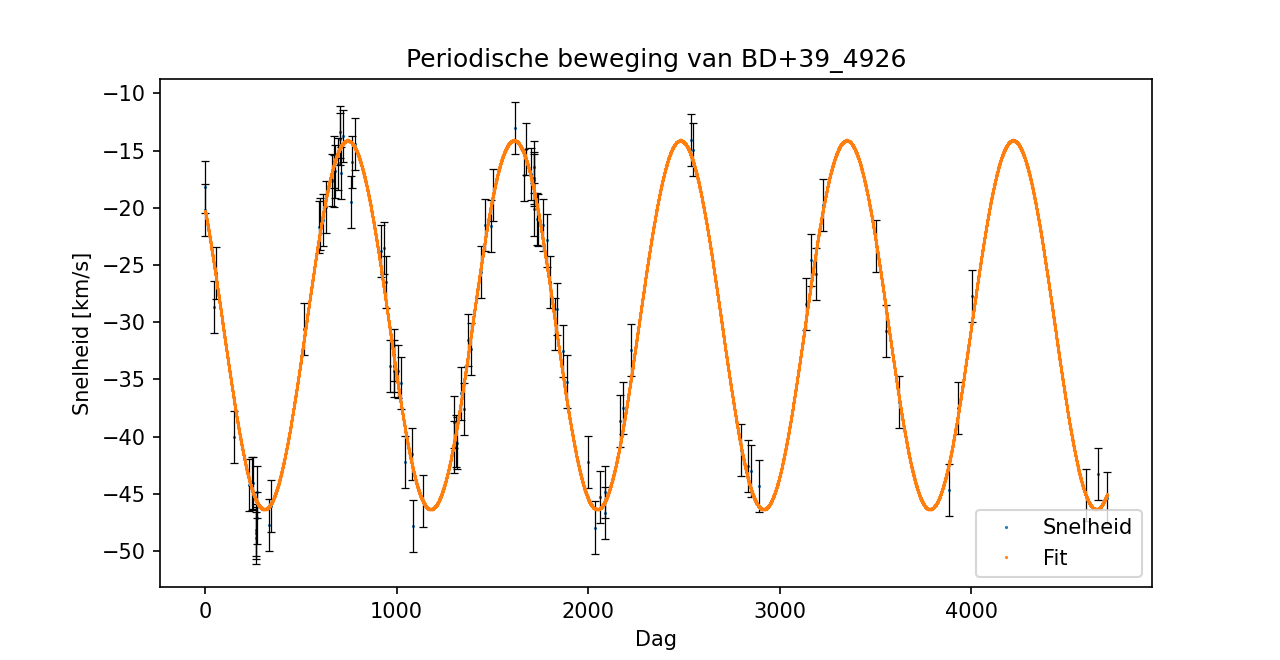
\includegraphics[width=1\textwidth]{snelheid per dag.png}
	    	\caption{Radiale snelheid in functie van dagen. De berekening van de fouten op de radiale snelheid wordt gegeven in appendix 1.}
	    	\label{fig 4:snelheid per dag}
	\end{figure}
	
	
	\pagebreak
	\noindent
	De massafunctie, $f(M)$, zoals bepaald in \eqref{massafunctie}, kan afgeleid worden uit de bewegingsvergelijking van een ECB:
	\begin{equation}
	F = \frac{m_1 v_1^2}{r_1}
	\end{equation}
	De massafunctie is een manier om de onmeetbare variabelen in functie van de meetbare variabelen te noteren, om zo deze variabelen te kunnen berekenen.
	Uit $f(M)$ en $m_1$, is $m_2$ in functie van de inclinatiehoek te bepalen. In dit geval is de $f(M)$ gelijk aan:
	\begin{equation}
		f(M) = 0.376 \,\textup{M}_\odot \pm 0.02\,\textup{M}_\odot
	\end{equation} 
	Ten slotte wordt de massa van de onzichtbare component, $m_2$, geplot in functie van de inclinatiehoek, zie figuur \ref{fig 5:massa ifv inclinatiehoek}.
	\begin{figure}[h]
		\centering
		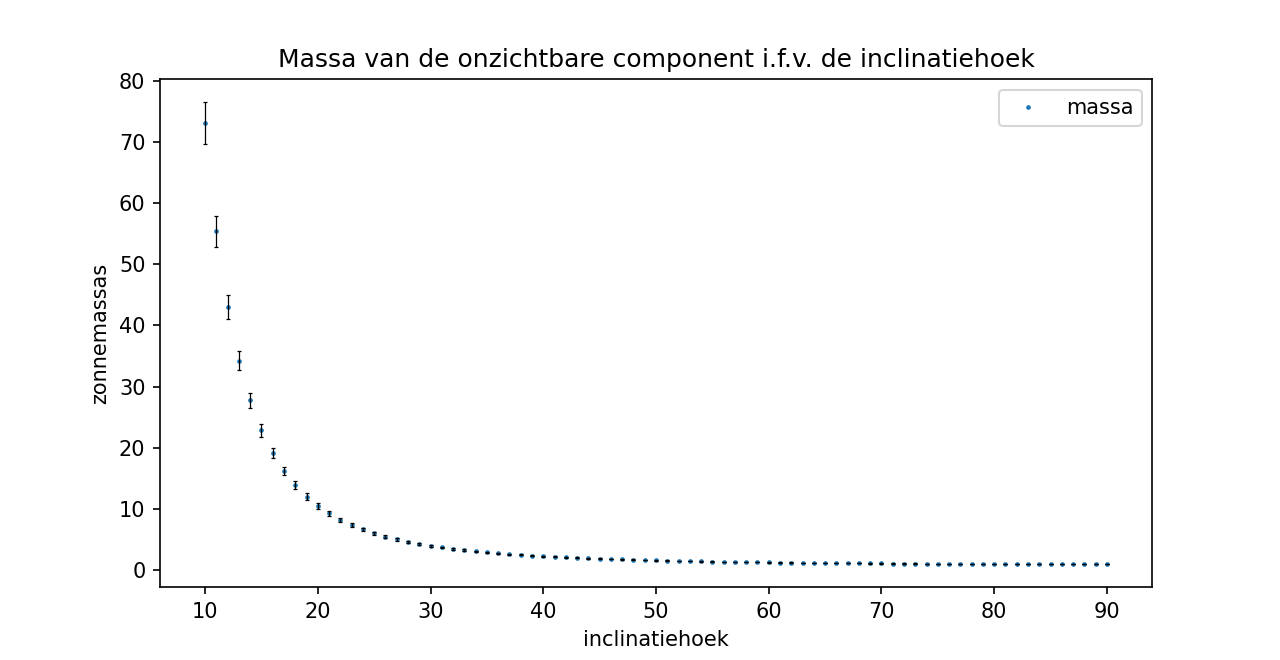
\includegraphics[width=0.8\textwidth]{massa ifv inclinatiehoek.png}
		\caption{Massa $m_2$ van de onzichtbare component i.f.v. de inclinatiehoek}
		\label{fig 5:massa ifv inclinatiehoek}
	\end{figure}
	\newpage
\section{Discussie}
In een uitdijnend heelal verwacht men eigenlijk een redshift te zien. Toch wordt hier een blueshift geobserveerd.
Dit betekent dus dat de dubbelster naar ons toe beweegt en wel met een radiale snelheid van $(30.2\,\pm0.2)\,km/s$.
 Ofwel gaat het dus om een dubbelstersysteem binnen de Melkweg dat een relatieve snelheid naar ons toe heeft; of een andere mogelijkheid is 
dat de dubbelster deel uitmaakt van een naburige sterrenstelsel dat naar ons toebeweegt, zoals bv. het Andromedasterrenstelsel. 
\\
In principe zou uit de bestudeerde datasets de massa van de onzichtbare component in het dubbelstersysteem kunnen bepaald worden. Hiervoor moet men wel de inclinatiehoek kennen. Daar deze informatie niet beschikbaar is, kan enkel een heel ruwe afschatting gemaakt worden. Voor realistische 
inclinatiehoeken tussen 20° en 90°, bekomt men een massa tussen 1 en 10 zonnemassa's.

\section{Conclusie}
Uit het waargenomen absorptiespectrum van de zichtbare component in het dubbelstersysteem BD+39\_4926, is a.d.h.v. de blauwverschuiving de radiale snelheid van de zichtbare component doorheen de tijd bepaald. Hieruit werd vervolgens de massa van de onzichtbare component bepaald in functie van de inclinatiehoek.
	
	

	\begin{thebibliography}{9}
		\bibitem{Opgave Sterrenkundeproef}  Van Winckel H., De Cock M., Opgave Sterrenkunde, internet, \textit{Toledo}, 13 November 2023
		%\bibitem{Cantor set} ANONIEM, Cantor set, internet, \textit{Wikipedia}, 13 November 2023, (https://en.wikipedia.org/wiki/Cantor\_set).
	\end{thebibliography}
\pagebreak

\section{Appendix 1: Foutberekeningen op v}

In deze bijlage worden de fouten op v berekend en beredeneerd.
\\\\
Eerst worden de fouten op de radiale snelheid berekend. Als er wordt aangenomen dat de fout op de intensiteit verwaarloosbaar is, dan kan een verschuivingsfactor $\mu$ gedefiniëerd worden als:
\begin{equation}
	\mu = \frac{\lambda}{\lambda_0} = 1 + \frac{v}{c}
\end{equation}
In dit geval is de fout op de lijst van absorptielijnen verwaarloosbaar. Dus:
\begin{equation}
	\Delta \mu = \frac{\Delta \lambda}{\lambda_0} = \Delta (1 + \frac{v}{c})
\end{equation}
Hieruit kan $\Delta v$ afgeleid worden. Dus:
\begin{equation}
	\Delta v = c \Delta \mu = c \frac{\Delta \lambda}{\lambda_0}
\end{equation}
Vervolgens is $\Delta \lambda$ berekenbaar via de resolutie van de spectrograaf als beschreven in \ref{spectrograaf}. Als volgt:
\begin{equation}
	\Delta \lambda = \frac{900 - 390}{168000} \text{nm}
\end{equation}
De minimale waarde voor $\lambda_0$ wordt gekozen, namelijk 400.025585, om een maximale fout op v te bekomen. Namelijk: $\Delta v = 2275.0651 \frac{m}{s}$
\\\\
Als er wordt aangenomen dat de fout op de intensiteit niet verwaarloosbaar is. Dan kan er voor elke uitgezonden golflengte $\lambda_0$ de waargenomen golflengte $\lambda$ berekend worden volgens:
\begin{equation}
	\lambda = (1 + \frac{v}{c})\lambda_0
\end{equation} 
Deze wordt berekend voor alle gegeven absorptielijnen. De lokale fouten op de intensiteit bij deze waarden worden bepaald door een verzameling van meetpunten rond de golflengte $\lambda$ te analyseren.
\begin{center}
	\begin{minipage}{1\textwidth}
		\begin{figure}[H]
			\centering
			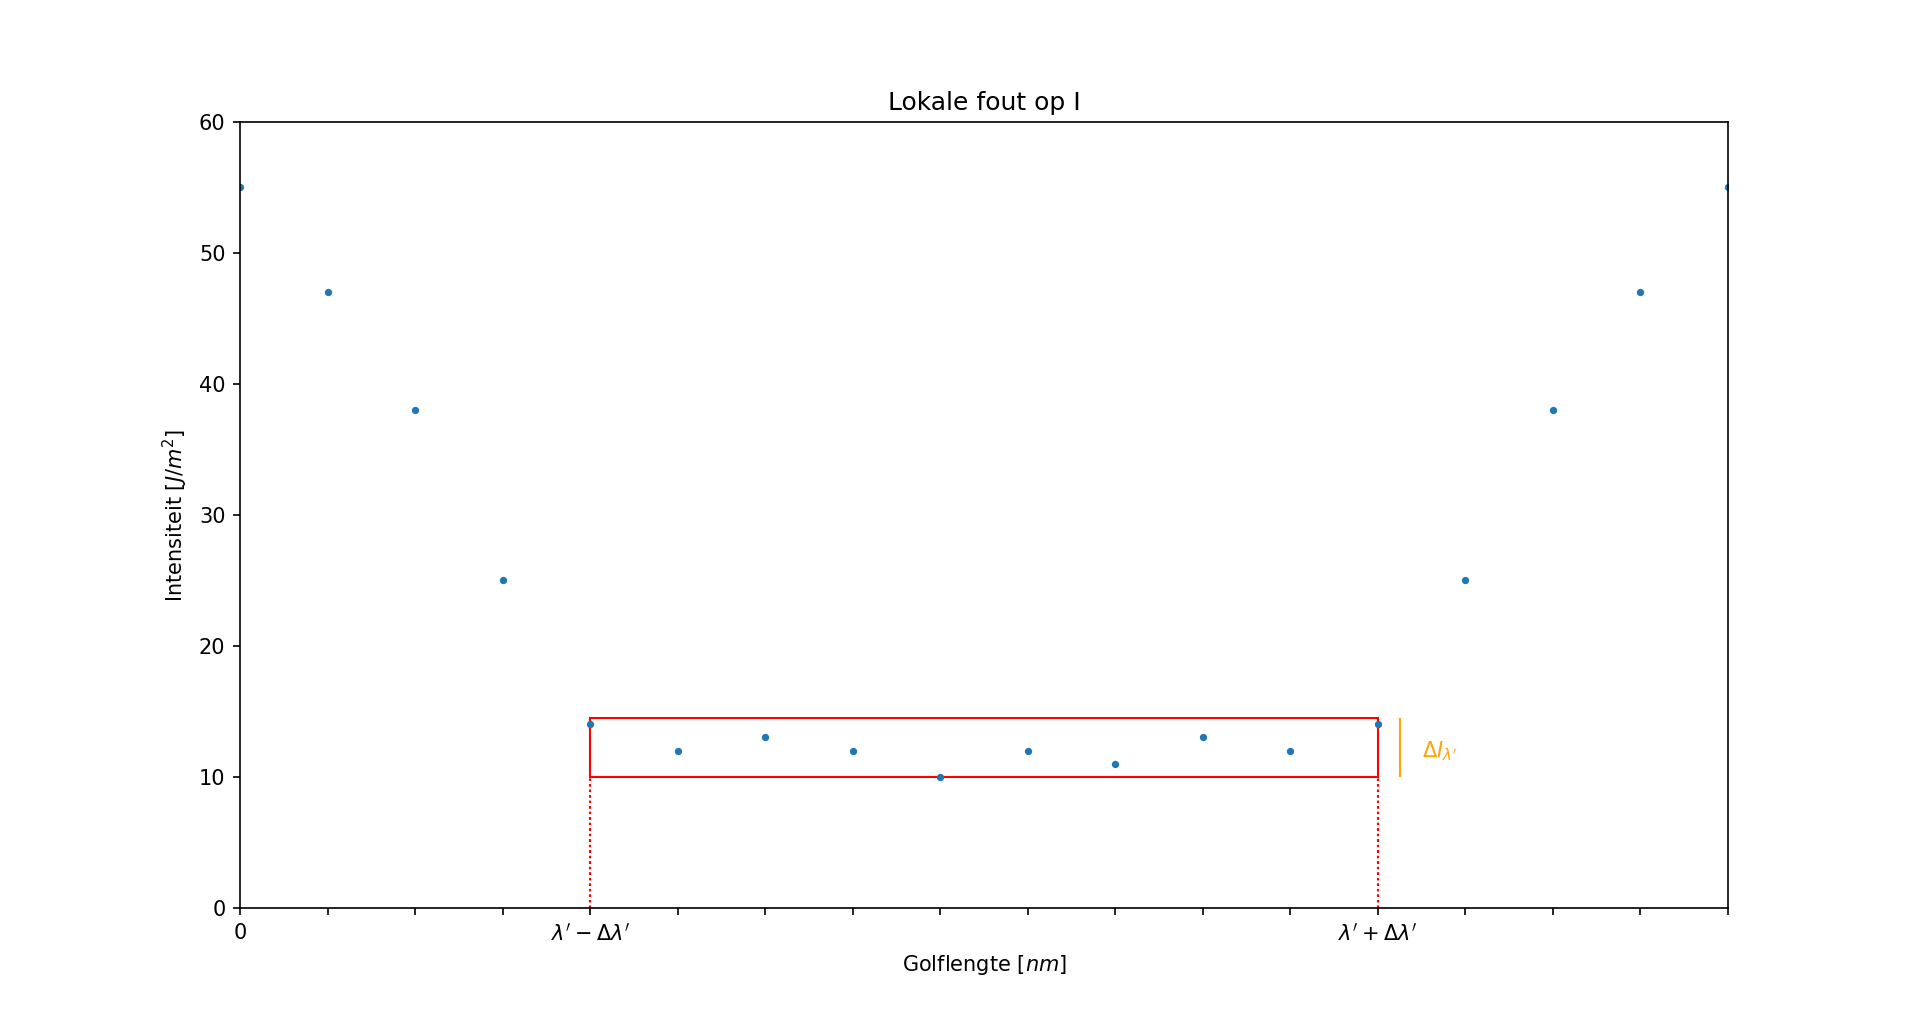
\includegraphics[width=1\textwidth]{lokale_fout_op_I.png}
			\caption{\label{fig 6: lokale fout op I} lokale fout op I}
		\end{figure}
	\end{minipage}
\end{center}
\noindent
Met de bekomen waarde voor $\Delta I_{\lambda '} $ wordt ook $\Delta som\,I$ bepaald en kan ook een interval, $[v-\Delta v, v+ \Delta v]$ gespecifiëerd worden. Dit interval is bepaald door voor voldoende $v$ de som van alle intensiteiten van de verschoven absorptielijnen te vergelijken.
\begin{center}
	\begin{minipage}{1\textwidth}
		\begin{figure}[H]
			\centering
			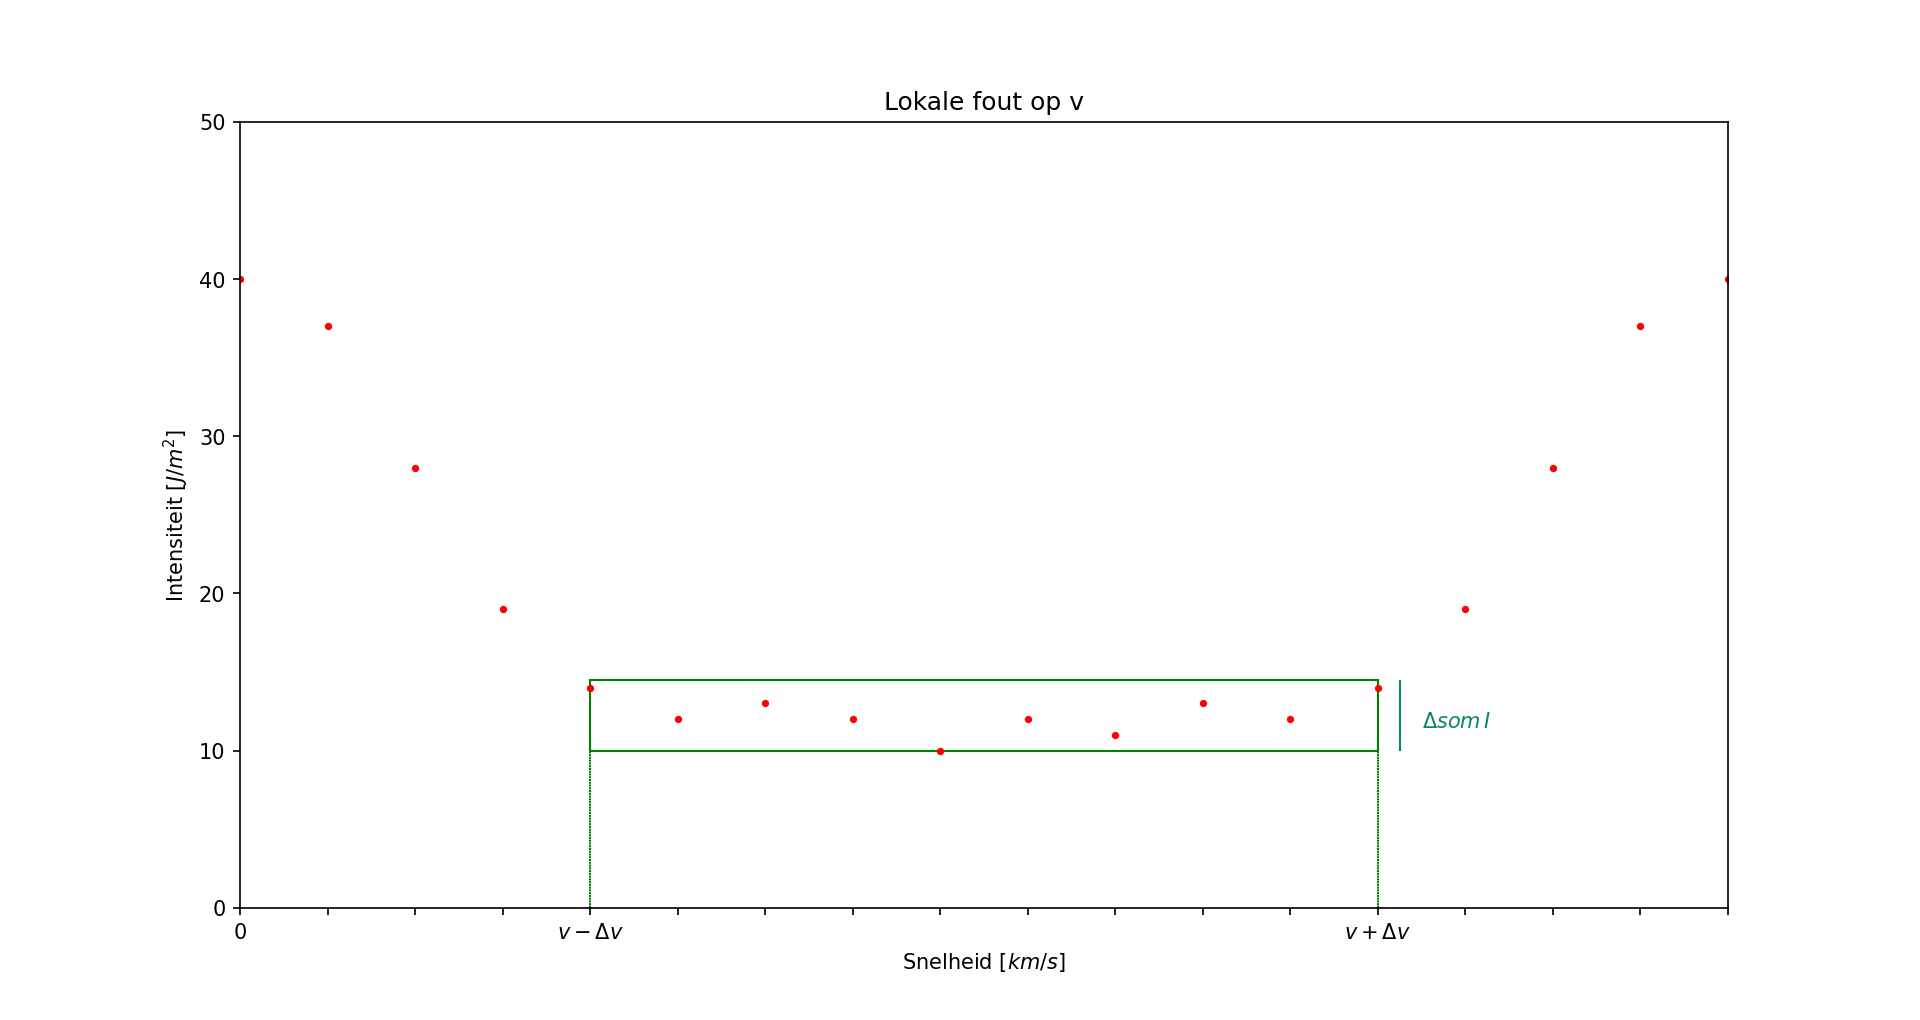
\includegraphics[width=1\textwidth]{lokale_fout_op_v.png}
			\caption{\label{fig 7: lokale fout op v} lokale fout op v}
		\end{figure}
	\end{minipage}
\end{center}
Deze figuren zijn een demonstratie van de gebruikte methodiek, niet de effectief bekomen data. Dit is omdat de $\Delta som\, I$ zodanig klein is dat de visualisatie de methodiek niet duidelijk maakt.\\
Hier kan door de doorwerkingsregel op de deelintensiteiten toe te passen (wetende dat deze in dezelfde grootteorde liggen) bevonden worden dat $O(\Delta som\, I) = O(\sqrt{N})$ met $N$ het aantal meetpunten terwijl $O(som\, I) = O(N)$. Waarbij O() een functie is die de grootteorde teruggeeft van het argument. Dus:
\begin{equation}
	\delta som\, I = \frac{\Delta som\, I}{ som\, I} \thickapprox \frac{\sqrt{N}}{N} = \frac{1}{\sqrt{N}} = \frac{1}{\sqrt{1944}} \thickapprox \frac{1}{44}
\end{equation}
Dit is kleiner dan het verschil tussen 2 meetpunten. Hieruit volgt dat $\Delta v$ als resultaat enkel en alleen van $\Delta I$ verwaarloosbaar is omdat de resolutie van de spectrograaf overschreden wordt.\\\\ 
Dit is te verwachten.
\\
De onzekerheid op de intensiteit verschuift elk minimum willekeurig. Maar de relatieve positie van alle minima is gekend, en een grotere verzameling van willekeurige verschuivingen resulteert in een kleinere standaardafwijking van de totale verschuiving. De fout op $v$ is dus gelijk aan de fout geïnduceerd door de resolutie van de spectrograaf wat geeft dat: $\Delta v = 2275.0651 \frac{m}{s}$
%\\\\
%De fout op de periode en de amplitude valt af te lezen uit de fit. De fout op de massafunctie wordt verkregen door de doorwerkingsregel toe te passen op het linkerlid van de vergelijking:
%\begin{equation}
%		\Delta f(M) = \Delta \frac{P v_{1v}^3}{2\pi} = \frac{v_{1r}^2}{2\pi} \sqrt{v_{1r}^2 (\Delta P)^2 + 9P^2 (\Delta v_{1r})^2}
%\end{equation}
\end{document}